93. $y=\cfrac{|x^2-5x+6|}{x-2}=\cfrac{|x-2||x-3|}{x-2}=\begin{cases} |x-3|, x>2,\\ -|x-3|, x<2.\end{cases}=\begin{cases} x-3,\ x\geqslant 3,\\ 3-x,\ 2<x<3,\\ x-3,\ x<2.\end{cases}$
$$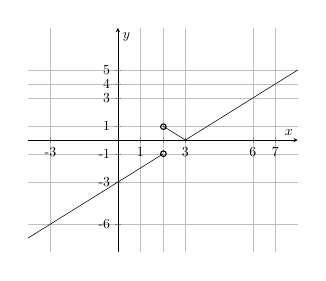
\begin{tikzpicture}[scale=0.5]
\begin{axis}[
    axis lines = middle,
    grid=major,
    legend pos={south west},
    xlabel = {$x$},
    ylabel = {$y$},
    ymin=-8,
    ymax=8,
    xtick={-3,1,2, 3,6,7},
    xticklabels={-3,1,$ $, 3,6,7},
    ytick={-6,-3,-1,1, 3,4,5},
    yticklabels={-6,-3,-1,1, 3,4,5}            ]
\addplot[domain=-4:2, samples=100, color=black] {-abs(x-3)};
\addplot[domain=2:8, samples=100, color=black] {abs(x-3)};
%\addplot[domain=-3.1:2.5, samples=100, color=red] {70*abs(1-2*abs(abs(x)-2))-10*x^2+10*x-70};
	%\addlegendentry{$\text{Рис. 1}$};
\end{axis}
\draw (3.44,3.185) circle (2pt);
\draw (3.44,2.5) circle (2pt);
\end{tikzpicture}$$
